\chapter{User interface}
\label{section:ui}

The application can be seen as a replacement for Exchange's web access, but also Outlook itself. When our
customers move from Microsoft's offering to Zarafa they want the transition to be as smooth as possible for
their end users. By providing an application that looks and feels like Outlook we minimise the learning 
curve for users, stimulating quick adoption.

\section{Overview}

The meat of the work is in developing a flexible user interface that presents \emph{items} (mail messages, 
appointments, tasks, contacts) to the user and lets the user create, manipulate, and exchange items with 
other users. There are three important aspects of the application that stimulate a high level of flexibility
and decoupling. 

\begin{itemize}
	\item{Outlook is a highly volatile application, 
	whose user interface changes radically at each major version. In order to keep up with new features added 
	to Outlook in the future, and to be able to add novel features of our own it is crucial that the interface
	architecture is not resistant to change and expansion.}
	\item{The application manages a variety of item types. 
	The application components that deal with these types have a low amount of interdependency, which
	makes it natural to develop them individually and concurrently.}
	\item{One of the requirements for the application is that it should be possible, and preferably easy,
	to develop third-party plug-ins.}
\end{itemize}

Ideally the application should be a loosely coupled group of components, where each component implements a sub-set 
of the functional requirements. We divide up the application into chunks called \emph{contexts}, each dealing with
a different entity type. Examples of contexts are the mail context, the calendar context, etc. This decoupling 
makes it possible to develop contexts independently on top of a global framework. The architecture is shown 
in Figure \ref{figure:architecture}.

\begin{figure}[h!]
\centering
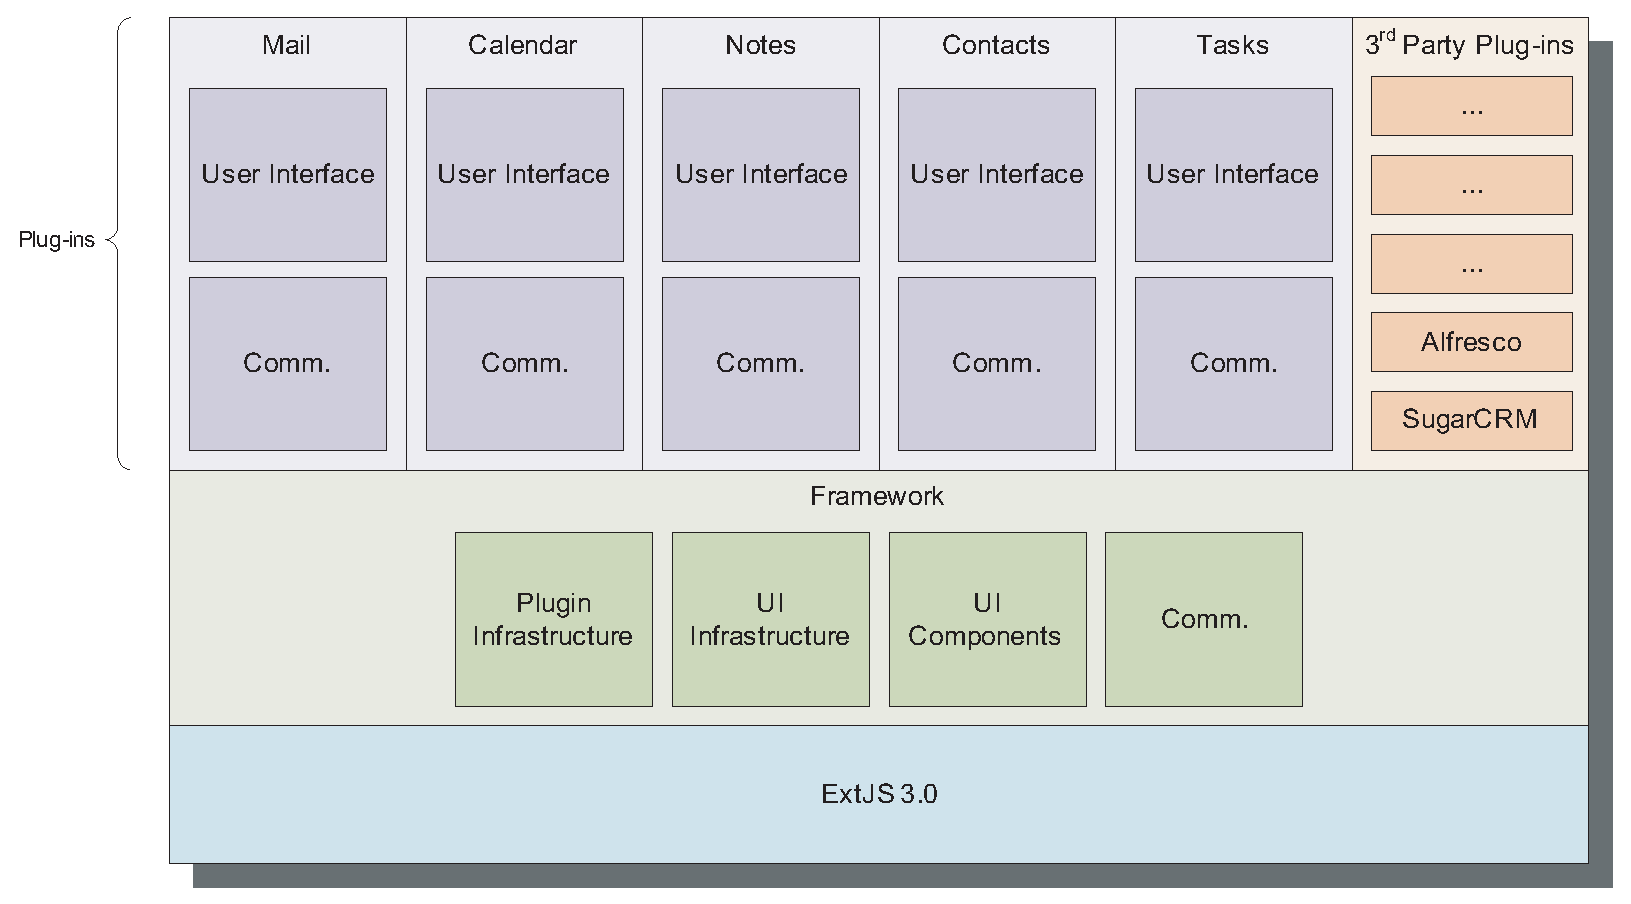
\includegraphics[width=14cm]{figures/stack.eps}
\caption{Architecture overview.}
\label{figure:architecture}
\end{figure}

The application framework sits atop the ExtJS 3.0 library and provides all the functionality that is needed across
contexts. The framework supports \emph{plug-ins}, functional components that can be added or removed at will. 
Contexts are implemented as plug-ins, and third-party developers can also develop their own to extend or 
customise the application.

The framework also provides a user interface infrastructure, with a main screen that carries all the standard
components that are used by all contexts. A set of custom user interface widgets such as a sophisticated
calendaring component are also included. Finally the framework supplies a communications API that allows
for both low-level and high-level interaction with the server-side back-end.

\section{Plug-ins}

The purpose of plug-ins is to have a way to add functionality to the application simply by adding additional
JavaScript files. 
Registered plug-ins can hook into so called \emph{insertion points} in the interface and register component
creation functions with them. This allows for a plug-in developer to easily add UI components such as buttons
or menu options to the application without modifying any 'core' code. 

A global object called {\tt container} manages, among other things, plug-ins. Plug-ins must extend {\tt Zarafa.ui.Plugin} 
and register a single instance with the container in order to be able to function. Plug-ins have unique names, by which
they can be identified and retrieved. 

Listing \ref{listing:exampleplugin} shows a bare-bones example plug-in. A new instance of the plug-in is created and
registered with the container on the last line of the code, using the {\tt registerPlugin} function. 
Note that the name of the plugin is a property of the
plugin itself, so there is no need to pass it when registering.

\begin{lstlisting}[caption={Example plugin.}, label=listing:exampleplugin]
// Ensure the 'Zarafa.plugins' namespace is declared.
Ext.namespace('Zarafa.plugins');

// Declare Zarafa.plugins.ExamplePlugin class.
Zarafa.plugins.ExamplePlugin = function()
{
	// Call parent constructor. Set plug-in name to 'example'.
	var config = { name : 'example' };
	Zarafa.plugins.ExamplePlugin.superclass.constructor.call(this, config);
};

// Express that the ExamplePlugin extends Plugin.
Ext.extend(Zarafa.plugins.ExamplePlugin, Zarafa.ui.Plugin, {
	
});

// Register a new instance of the plugin with the global container.
container.registerPlugin(new Zarafa.plugins.ExamplePlugin());\end{lstlisting}

\section{Contexts}
\label{section:contexts}

As discussed, functionality for working with different item types is encapsulated
in various contexts. Each context is a special type of plug-in that has additional functionality allowing it to 
'take over' the toolbar and main content section of application screen. Folders in the folder hierarchy are 
linked to contexts that display their contents, so that when a user clicks his or her inbox, the mail context
is enabled. 

The main application screen consists of several standard areas, shown in Figure \ref{figure:layout}.
The UI provides a standard hierarchy panel showing a list of folders the user has access to, as well as a 
bottom tool bar. Each context has its own content panel and tool bar, but only the ones belonging to the 
currently active context are visible while all others are hidden. This is achieved by loading the tool bars 
and content panels of all contexts into their respective areas and using card layouts to switch between them.

\begin{figure}[h!]
\centering
\includegraphics[width=10cm]{figures/layout.eps}
\caption{Screen layout.}
\label{figure:layout}
\end{figure}

Generally a context switch is performed when the user selects a folder from the hierarchy tree at the left
of the screen. A simple bidding mechanism is in place to determine which context will be used to show that
folder. Each content context implements a {\tt bid()} method that is passed store and folder details and
returns a numerical value indicating how well it is able to handle that folder type. The content context
that bids the highest is then selected.

\section{Insertion points}
\label{section:insertionpoints}

An \emph{insertion point} is a named location in the UI component hierarchy where plug-ins may add components. 
Insertion points are typically added to tool bars and context menus, and are intented as easy hooks for adding 
new buttons or menu items.

Plug-ins register functions with insertion points. When the application starts and the UI is constructed, 
these functions will be called automatically. They may return one or more UI components, which will be added 
to the hierarchy at the appropriate locations.

\subsection{Creating insertion points}

Insertion points are implemented as a call to the container, which collects UI components from registered
plug-ins and returns them. Listing \ref{listing:insertionpoints} shows how to create an insertion point. 

\begin{lstlisting}[caption={Insertion point.}, label=listing:insertionpoints]
function createToolbar()
{

	return new Ext.Toolbar(
	{

		items : [
				{
					iconCls : 'icon_delete',
				},
				{
					iconCls : 'icon_copy'
				},
				{
					iconCls : 'icon_print'
				},
				{
					iconCls : 'icon_addressbook'
				}, 
				'-',
				// insertion point 'example.toolbar'
				container.populateInsertionPoint('example.toolbar')
		]

	});
}
\end{lstlisting}

By design the names of the insertion points should reflect the structure of the application. Therefore
the proposed naming scheme follows a hierarchy separated by dot ('.') characters. For example, the
top tool bar of the 'tasks' context is called {\tt context.tasks.toolbar}. Insertion points may be contained 
in right-click menus (ie {\tt main.hierarchy.contextmenu}), dialogs (ie {\tt dialogs.properties.toolbar}),
and may even be nested.

Insertion points are supported by the documentation tool and should be documented for easy reference. More
on this in Section \ref{section:docinsert}.

\subsection{Using insertion points}

An example plug-in that adds a 'hello world' button to the toolbar is shown in Listing \ref{listing:exampleplugin2}. 
The plug-in registers the {\tt createButton} function with the {\tt example.toolbar} insertion point (line 9). 

\begin{lstlisting}[caption={Using an insertion point.}, label=listing:exampleplugin2]
Ext.namespace('Zarafa.plugins');

Zarafa.plugins.ExamplePlugin = function()
{
	config = { name : 'example' };
	Zarafa.plugins.ExamplePlugin.superclass.constructor.call(this, config);
	
	// register the 'createButton' method with the 'example.toolbar' insertion point.
	this.registerInsertionPoint('example.toolbar', this.createButton, this);
};

Ext.extend(Zarafa.plugins.ExamplePlugin, Zarafa.ui.Plugin, {
	
	// Creates a single button that pops up a 'Hello world!' message when clicked.
	createButton : function(insertionPoint)
	{
		return new Ext.Button({
			text : 'Hello!',
			handler : function()
			{
				alert('Hello world!');
			}
		});
	}	
	
});

container.registerPlugin(new Zarafa.plugins.ExamplePlugin());\end{lstlisting}

The function {\tt registerInsertionPoint(match, func, scope)} registers a function 'func' so that it is 
called when an insertion point 'match' is populated. The function should return one or more UI components
({\tt Ext.Component} instances). Note that the 'match' parameter can be either a {\tt string} denoting
the name of the insertion point, or a regular expression to match multiple insertion points.

It's possible to hook into several insertion points explicitly by registering each one separately,
or by using a regular expression. Listing \ref{listing:insertregexp} shows how the code from
Listing \ref{listing:exampleplugin2} could be altered to create a button on the tool bars
of all contexts. The match parameter has been changed to a regular expression that matches 
'context.mail.toolbar', 'context.notes.toolbar', etc.

\begin{lstlisting}[caption={Matching with regular expressions.}, label=listing:insertregexp]
this.registerInsertionPoint(/context\..*?\.toolbar/, this.createButton, this);\end{lstlisting}
 
\subsection{Parameters}

In some cases it's useful to have insertion points that provide extra information to the plug-in. An example 
is an insertion point in a context menu, where it's useful to pass the menu object ({\tt Ext.menu.Menu}) to the
creation function. Another example is a toolbar in a 'read mail' dialog, which might pass the entry ID of the 
item that is being shown to the plug-in. 

The modified insertion point declaration and button creation function are shown in Listing 
\ref{listing:insertionpoints2} and \ref{listing:exampleplugin3} respectively.

\begin{lstlisting}[caption={Insertion point with parameter.}, label=listing:insertionpoints2]
container.populateInsertionPoint('dialog.readmail.toolbar', mailEntryId);
\end{lstlisting}

\begin{lstlisting}[caption={Using an insertion point with parameters.}, label=listing:exampleplugin3]
createButton : function(insertionPoint, messageEntryId)
{
	return new Ext.Button({
		text : 'Hello!',
		handler : function()
		{
			alert('Message ID: ' + messageEntryId);
		}
	});
}	
container.registerPlugin(new Zarafa.plugins.ExamplePlugin());\end{lstlisting}





